
\providecommand{\rvC}{\mathbf{C}}  %
\providecommand{\rvW}{\mathbf{W}}  %
\providecommand{\rvF}{\mathbf{F}}  %
\providecommand{\rvWarrow}{\rightsquigarrow}%
\providecommand{\rvFarrow}{\twoheadrightarrow}%
\providecommand{\rvTFarrow}{\rightsquigarrow\joinrel\twoheadrightarrow}%
\providecommand{\rvCarrow}{\rightarrowtail}%
\providecommand{\rvTCarrow}{\rightarrowtail\joinrel\rightsquigarrow}%

\section{模型范畴与 Quillen 函子}\label{sec:model-categories-and-quillen-functors}

下面对 Quillen 的「闭模型范畴」（closed model category）定义%
\cite[I.5.1.1]{bib93} 的重新表述由 Joyal 与 Tierney 给出 \cite[7.7]{bib64}，他们%
证明了：一个配有满足\trTwoOfThreeProperty{}的\trWeakEquivalence{}的\trCategory{}
$(\mathcal{M},\rvW)$ 容有一个\trModelStructure，恰在存在定义如下一对%
\trWeakFactorizationSystem{}的类 $\rvC$ 与 $\rvF$ 时：

\begin{definition}[模型范畴]\label{def:model-structure}
一个\trComplete{}且\trCocomplete{}的\trCategory{} $\mathcal{M}$ 上的一个%
\textbf{\trModelStructure}由映射的三个类构成——\textbf{\trWeakEquivalence}
$\rvW$（记作「$\rvWarrow$」），它必须满足\trTwoOfThreeProperty；\textbf{余纤维
化}（cofibration）$\rvC$（记作「$\rvCarrow$」）；以及\textbf{\trFibration}
$\rvF$（记作「$\rvFarrow$」）——使得 $(\rvC,\rvF\cap\rvW)$ 与
$(\rvC\cap\rvW,\rvF)$ 各自在 $\mathcal{M}$ 上定义一个\trWeakFactorizationSystem。%
\footnote{在\trModelCategory{}的诸标准定义中有一条公理——\trWeakEquivalence{}对%
\trRetract{}的封闭性——并未显然地被打包进这些假设之中，但它是此处所给诸公理的
一个推论 \cite[7.8]{bib64}。}

一个\textbf{\trModelCategory}是一个配有\trModelStructure{}的\trComplete{}且%
\trCocomplete{}的\trCategory。\trModelCategory{}中表现更佳的对象或「\trFibrant」、
或「\trCofibrant」、或两者兼备：
\end{definition}

\begin{definition}\label{def:fibrant-cofibrant}
在\trModelCategory{} $\mathcal{M}$ 中，一个对象 $X$ 是\textbf{\trFibrant}的，恰在%
从它到\trTerminal{}对象的唯一映射 $X\to 1$ 是一支\trFibration{}时；是%
\textbf{\trCofibrant}的，恰在从\trInitial{}对象出发的唯一映射%
$\varnothing\to X$ 是一支余纤维化时。经由分解这些唯一映射，任何对象 $X$ 都拥有按
如下方式构造的一个\textbf{余纤维性替换}（cofibrant replacement）$QX$ 与一个%
\textbf{纤维性替换}（fibrant replacement）$RX$：
\begin{center}
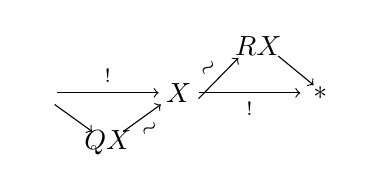
\begin{tikzpicture}[x=1.6em,y=1.4em]
  \node (RX) at (5.0,2.5) {$RX$};
  \node (empty) at (0,1.3) {$\varnothing$};
  \node (X) at (3.2,1.3) {$X$};
  \node (star) at (6.4,1.3) {$\ast$};
  \node (QX) at (1.6,0) {$QX$};
  \draw[->] (0.45,1.3) -- (2.75,1.3);
  \node at (1.6,1.74) {$\scriptstyle !$};
  \draw[->] (3.65,1.15) -- (4.55,2.2) node[midway,above,sloped]{$\scriptstyle\sim$};
  \draw[->] (5.45,2.25) -- (6.25,1.5);
  \draw[->] (3.65,1.3) -- (5.95,1.3);
  \node at (4.8,0.9) {$\scriptstyle !$};
  \draw[->] (0.4,1.0) -- (1.25,0.3);
  \draw[->] (1.95,0.3) -- (2.8,1.0) node[midway,below,sloped]{$\scriptstyle\sim$};
\end{tikzpicture}
\end{center}
\end{definition}

请注意，\cref{def:weak-factorization-system}与\cref{def:model-structure}是自对
偶的：若 $(\mathrm{L},\mathrm{R})$ 定义 $\mathcal{M}$ 上的一个\trWeakFactorizationSystem，则
$(\mathrm{R},\mathrm{L})$ 定义 $\mathcal{M}^{\mathrm{op}}$ 上的一个\trWeakFactorizationSystem。
于是，关于\trFibration{}之右类 $\rvF$ 与\textbf{\trTrivialFibration}%
「$\rvTFarrow$」之右类 $\rvF\cap\rvW$ 的一切一般性定理，都蕴涵涉及余纤维化之左类
$\rvC$ 与\textbf{平凡余纤维化}（trivial cofibration）「$\rvTCarrow$」之左类
$\rvC\cap\rvW$ 的诸对偶结果。特别地，由\cref{exa:model-category-fibrant-objects}，
C.1 节中所证明的关于一个\trCategoryOfFibrantObjects{}的全部结果，对于\trModelCategory{}中由此
得名的诸\trFibrant{}对象之间的\trFibration、\trTrivialFibration{}与%
\trWeakEquivalence{}都成立，而这些结果的诸对偶对于\trCofibrant{}对象之间的余纤
维化、平凡余纤维化与\trWeakEquivalence{}亦成立。

还请注意：既然\trWeakFactorizationSystem{}的任何一个类都确定另一个类，平凡余纤维化便可以在既不参
照余纤维化也不参照\trWeakEquivalence{}的情况下定义出来——即那些对诸%
\trFibration{}具有左\trLifting{}性质的映射；对偶地，\trTrivialFibration{}恰是那
些对诸余纤维化具有右\trLifting{}性质的映射。

\begin{definition}\label{def:quillen-functor}
介于诸\trModelCategory{}之间的一个\trFunctor{}是
\begin{itemize}
\item \textbf{左 Quillen}的，若它保持余纤维化、平凡余纤维化与\trCofibrant{}对
  象；并且
\item \textbf{右 Quillen}的，若它保持\trFibration、\trTrivialFibration{}与%
\trFibrant{}对象。
\end{itemize}
\end{definition}

左 Quillen \trFunctor{}容有左导出函子，而右 Quillen \trFunctor{}容有右导出函子。
为免于定义这些术语，我们把这方面的完整论述留给其他作者 \cite[§2.1--2]{bib103}，
但 Quillen \trFunctor{}之「可导出性」的一个重要成分已由下述结果所捕捉：

\begin{lemma}\label{lem:quillen-preserves-we}
介于诸\trModelCategory{}之间的任何左 Quillen \trFunctor{}都保持\trCofibrant{}对
象之间的\trWeakEquivalence，而任何右 Quillen \trFunctor{}都保持\trFibrant{}对象
之间的\trWeakEquivalence。
\end{lemma}
\begin{proof}
对右 Quillen \trFunctor{}而言，这直接由\cref{lem:ken-brown}与%
\cref{exa:model-category-fibrant-objects}得出。左 Quillen \trFunctor{}的结果是对
偶的。
\end{proof}

大多数左 Quillen \trFunctor{}都是「余连续的」，保持一切\trColimit；而大多数右
Quillen \trFunctor{}都是「连续的」，保持一切\trLimit；当情形如此时，便无须另行
假设\trCofibrant{}对象或\trFibrant{}对象被保持。事实上，Quillen \trFunctor{}通常
以\trAdjunction{}对的形态出现：

\begin{definition}\label{def:quillen-adjunction}
试考虑介于一对\trModelCategory{}之间的一个\trAdjunction
\begin{center}
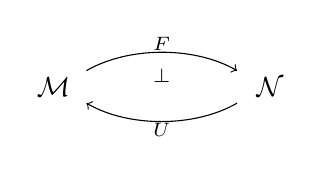
\begin{tikzpicture}[x=1.7em,y=1.4em]
  \node (M) at (0,0) {$\mathcal{M}$};
  \node (N) at (4.6,0) {$\mathcal{N}$};
  \draw[->] (0.7,0.42) .. controls (1.6,1.05) and (3.0,1.05) .. (3.9,0.42);
  \node at (2.3,1.12) {$\scriptstyle F$};
  \node at (2.3,0.28) {$\scriptstyle\bot$};
  \draw[->] (3.9,-0.42) .. controls (3.0,-1.05) and (1.6,-1.05) .. (0.7,-0.42);
  \node at (2.3,-1.12) {$\scriptstyle U$};
\end{tikzpicture}
\end{center}
由\cref{lem:adjunction-transposes-lifting}，下列诸条件等价，它们定义一个%
\textbf{Quillen \trAdjunction}（Quillen adjunction）：
\begin{enumerate}[label=(\roman*)]
\item \trLeftAdjoint{} $F$ 是左 Quillen 的。
\item \trRightAdjoint{} $U$ 是右 Quillen 的。
\item \trLeftAdjoint{}保持余纤维化，而\trRightAdjoint{}保持\trFibration。
\item \trLeftAdjoint{}保持平凡余纤维化，而\trRightAdjoint{}保持%
\trTrivialFibration。
\end{enumerate}
\end{definition}

\begin{lemma}\label{lem:quillen-equivalence}
对于一个 Quillen \trAdjunction
\begin{center}
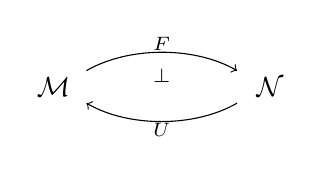
\begin{tikzpicture}[x=1.7em,y=1.4em]
  \node (M) at (0,0) {$\mathcal{M}$};
  \node (N) at (4.6,0) {$\mathcal{N}$};
  \draw[->] (0.7,0.42) .. controls (1.6,1.05) and (3.0,1.05) .. (3.9,0.42);
  \node at (2.3,1.12) {$\scriptstyle F$};
  \node at (2.3,0.28) {$\scriptstyle\bot$};
  \draw[->] (3.9,-0.42) .. controls (3.0,-1.05) and (1.6,-1.05) .. (0.7,-0.42);
  \node at (2.3,-1.12) {$\scriptstyle U$};
\end{tikzpicture}
\end{center}
下列诸条件等价，并且刻画了那些定义\textbf{Quillen \trEquivalence}（Quillen
equivalence）的 Quillen \trAdjunction：
\begin{enumerate}[label=(\roman*)]
\item 对每个\trCofibrant{}对象 $M\in\mathcal{M}$ 与每个\trFibrant{}对象
  $N\in\mathcal{N}$，映射 $f^{\sharp}\colon FM\to N$ 是 $\mathcal{N}$ 中的%
\trWeakEquivalence，当且仅当其转置 $f^{\flat}\colon M\to UN$ 是 $\mathcal{M}$ 中
的\trWeakEquivalence。
\item 对每个\trCofibrant{}对象 $M\in\mathcal{M}$，导出单位（derived unit）
  \[ M\xrightarrow{\ \eta\ }UFM\longrightarrow URFM \]
  ——由\trUnit{}与纤维性替换复合而定义——是\trWeakEquivalence；并且对每个%
\trFibrant{}对象 $N\in\mathcal{N}$，导出余单位（derived counit）
  \[ FQUN\longrightarrow FUN\xrightarrow{\ \varepsilon\ }N \]
  ——由\trCounit{}与余纤维性替换复合而定义——是\trWeakEquivalence。
\end{enumerate}
\end{lemma}

\begin{proof}
假设 (i) 成立，并试考虑一个\trCofibrant{}对象 $M\in\mathcal{M}$ 与一个%
\trFibrant{}对象 $N\in\mathcal{N}$。导出单位与导出余单位分别是纤维性替换映射与余
纤维性替换映射的转置
\[ FM\;\rvWarrow\;RFM \qquad\qquad QUN\;\rvWarrow\;UN \]
由\cref{def:fibrant-cofibrant}，这些映射是\trWeakEquivalence；既然 $M$ 与 $QUN$
是\trCofibrant{}的而 $RFM$ 与 $N$ 是\trFibrant{}的，(i) 便告诉我们：导出单位与导
出余单位也必是\trWeakEquivalence。

现在假设导出单位是\trWeakEquivalence，并试考虑\trWeakEquivalence{}
$f^{\sharp}\colon FM\rvWarrow N$，其中 $M$ 是\trCofibrant{}的而 $N$ 是%
\trFibrant{}的。施用\trRightAdjoint{}与纤维性替换，我们得到一个交换\trDiagram
\begin{center}
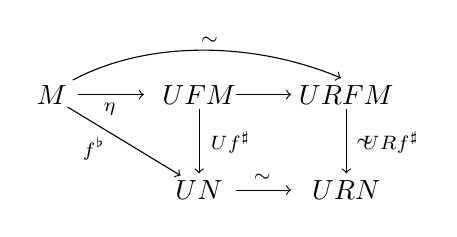
\begin{tikzpicture}[x=1.9em,y=1.5em]
  \node (M) at (0,2.3) {$M$};
  \node (UFM) at (2.8,2.3) {$UFM$};
  \node (URFM) at (5.6,2.3) {$URFM$};
  \node (UN) at (2.8,0) {$UN$};
  \node (URN) at (5.6,0) {$URN$};
  \draw[->] (0.5,2.3) -- (1.75,2.3);
  \node at (1.1,1.95) {$\scriptstyle\eta$};
  \draw[->] (3.5,2.3) -- (4.55,2.3);
  \draw[->] (0.4,2.65) .. controls (1.8,3.6) and (3.8,3.6) .. (5.5,2.7);
  \node at (3.0,3.6) {$\scriptstyle\sim$};
  \draw[->] (0.3,2.0) -- (2.45,0.35);
  \node at (0.8,1.0) {$\scriptstyle f^{\flat}$};
  \draw[->] (2.8,1.95) -- (2.8,0.4);
  \node at (3.4,1.15) {$\scriptstyle Uf^{\sharp}$};
  \draw[->] (5.6,1.95) -- (5.6,0.4);
  \node at (5.95,1.15) {$\scriptstyle\sim$};
  \node at (6.45,1.15) {$\scriptstyle URf^{\sharp}$};
  \draw[->] (3.5,0) -- (4.55,0);
  \node at (4.0,0.3) {$\scriptstyle\sim$};
\end{tikzpicture}
\end{center}
由\cref{lem:quillen-preserves-we}，右边与底部的映射是\trWeakEquivalence，而由假
设，作为顶部复合出现的导出单位亦然。由\trTwoOfThreeProperty，转置
$f^{\flat}\colon M\rvWarrow UN$ 也是\trWeakEquivalence。对偶地，若导出余单位是%
\trWeakEquivalence，则\trWeakEquivalence{} $f^{\flat}\colon M\rvWarrow UN$ 经转
置给出\trWeakEquivalence{} $f^{\sharp}\colon FM\rvWarrow N$。
\end{proof}

现在我们在\trDiagram{}\trCategory{}上引入一对\trModelStructure，其设计用意在于
保证对角\trFunctor{} $\Delta\colon\mathcal{M}\to\mathcal{M}^{\mathcal{J}}$ 分别
是右 Quillen 的或左 Quillen 的，从而\trColimit{}\trFunctor{}与\trLimit{}\trFunctor{}%
分别是左 Quillen 的或右 Quillen 的。相应的左、右导出函子随后便定义%
\textbf{\trHomotopyColimit}（homotopy colimit）与\textbf{\trHomotopyLimit}
（homotopy limit）\trFunctor。

\begin{definition}\label{def:projective-injective-model-structures}
设 $\mathcal{M}$ 是一个\trModelCategory，并设 $\mathcal{J}$ 是一个小范畴（small
category）。
\begin{enumerate}[label=(\roman*)]
\item $\mathcal{M}^{\mathcal{J}}$ 上的\textbf{射影模型结构}（projective model
  structure）的\trWeakEquivalence{}与\trFibration{}在 $\mathcal{M}$ 中逐点定义。
\item $\mathcal{M}^{\mathcal{J}}$ 上的\textbf{\trInjectiveModelStructure}（injective model
  structure）的\trWeakEquivalence{}与余纤维化在 $\mathcal{M}$ 中逐点定义。
\end{enumerate}
\end{definition}

当\trModelCategory{} $\mathcal{M}$ 是\emph{组合的}（combinatorial）或更一般的%
\emph{\trAccessible}（accessible）时，射影与\trInjectiveModelStructure{}总是存在 \cite{bib54}。
当然，即便没有这些假设，射影与\trInjectiveModelStructure{}也可能碰巧存在于
$\mathcal{M}^{\mathcal{J}}$ 之上——或许对特定的\trDiagram{}形状 $\mathcal{J}$
如此。

一个 Quillen 双变量伴随是这样的双变量\trAdjunction：其\trLeftAdjoint{}是一个左
Quillen \trBifunctor，而其诸\trRightAdjoint{}都是右 Quillen \trBifunctor。由%
\cref{ex:leibniz-lifting-equivalences}，这些条件中的任何一个都蕴涵其余两个：

\begin{definition}\label{def:quillen-two-variable-adjunction}
一个双变量\trAdjunction
\[ \mathcal{V}\times\mathcal{M}\xrightarrow{\ \otimes\ }\mathcal{N},\qquad
   \mathcal{V}^{\mathrm{op}}\times\mathcal{N}\xrightarrow{\ \{,\}\ }\mathcal{M},
   \qquad
   \mathcal{M}^{\mathrm{op}}\times\mathcal{N}\xrightarrow{\ \mathrm{hom}\ }\mathcal{V} \]
介于\trModelCategory{} $\mathcal{V}$、$\mathcal{M}$ 与 $\mathcal{N}$ 之间。若下
列等价条件中的任何一个——从而全部——得到满足，则它定义一个\textbf{Quillen 双
变量\trAdjunction}（Quillen two-variable adjunction）：
\begin{enumerate}[label=(\roman*)]
\item \trFunctor{} $\widehat{\otimes}\colon\mathcal{V}^{\mathbf{2}}\times\mathcal{M}^{\mathbf{2}}\to\mathcal{N}^{\mathbf{2}}$ 把 $\mathcal{V}$ 中一支余
  纤维化与 $\mathcal{M}$ 中一支余纤维化载为 $\mathcal{N}$ 中一支余纤维化，进而当
  两支定义域余纤维化中有任何一支是\trWeakEquivalence{}时，这支余纤维化也是%
\trWeakEquivalence。
\item \trFunctor{} $\widehat{\{,\}}\colon(\mathcal{V}^{\mathbf{2}})^{\mathrm{op}}\times\mathcal{N}^{\mathbf{2}}\to\mathcal{M}^{\mathbf{2}}$ 把 $\mathcal{V}$ 中一支余
  纤维化与 $\mathcal{N}$ 中一支\trFibration{}载为 $\mathcal{M}$ 中一支%
\trFibration，进而当两支定义域映射中有任何一支是\trWeakEquivalence{}时，这支%
\trFibration{}也是\trWeakEquivalence。%
  \footnote{原书于此印作「to a fibration in $\mathcal{N}$」；按该函子之值域为
  $\mathcal{M}^{\mathbf{2}}$，疑为 $\mathcal{M}$ 之误，此处径改。——译者注}
\item \trFunctor{} $\widehat{\mathrm{hom}}\colon(\mathcal{M}^{\mathbf{2}})^{\mathrm{op}}\times\mathcal{N}^{\mathbf{2}}\to\mathcal{V}^{\mathbf{2}}$ 把 $\mathcal{M}$ 中
  一支余纤维化与 $\mathcal{N}$ 中一支\trFibration{}载为 $\mathcal{V}$ 中一支%
\trFibration，进而当两支定义域映射中有任何一支是\trWeakEquivalence{}时，这支%
\trFibration{}也是\trWeakEquivalence。
\end{enumerate}
\end{definition}

\begin{remark}\label{rem:left-quillen-bifunctor}
由\cref{def:quillen-two-variable-adjunction}，一个双变量\trAdjunction{}是 Quillen
的，当且仅当其\trLeftAdjoint{} $\otimes\colon\mathcal{V}\times\mathcal{M}\to\mathcal{N}$
是一个\textbf{左 Quillen \trBifunctor}（left Quillen bifunctor）：
一个相对于诸构成性\trWeakFactorizationSystem{}的八种可能选取中的七种为左 Leibniz 的%
\trBifunctor——唯一的例外是对 $\mathcal{V}$ 与 $\mathcal{M}$ 都选取
$(\rvC,\rvF\cap\rvW)$、而对 $\mathcal{N}$ 选取 $(\rvC\cap\rvW,\rvF)$ 的那一种
选取。
\end{remark}

Quillen 对其单纯集范畴上的\trModelStructure{}所享有的附加性质所作的公理化，已被
Hovey \cite[§4.2]{bib57} 加以推广，以定义幺半模型范畴与富集模型范畴的概念。我们
把前者特化到 A.1 节的那些\trCartesianClosed{}范畴——因为此处需要的只有这些情形。
若 $\mathcal{V}$ 具有一个\trModelStructure、同时也是一个\trCartesianClosed{}范
畴，则自然要问这些结构是否相容，其意义如下：

\begin{definition}\label{def:cartesian-closed-model-category}
一个\textbf{笛卡尔封闭的模型范畴}（cartesian closed model category）是一个%
\trCartesianClosed{}范畴 $(\mathcal{V},\times,1)$ 配上一个\trModelStructure，使得
\begin{enumerate}[label=(\roman*)]
\item \trCartesianProduct{}与\trInternalHom{}定义一个 Quillen 双变量\trAdjunction；并且
\item 由\trTerminal{}对象的余纤维性替换所定义的映射
  $Q1\times v\to 1\times v\cong v$，在 $v$ 是\trCofibrant{}的时是%
\trWeakEquivalence。
\end{enumerate}
\end{definition}

\begin{definition}\label{def:v-model-category}
若 $\mathcal{V}$ 是一个笛卡尔封闭的模型范畴，则一个\textbf{$\mathcal{V}$-模型范
畴}（$\mathcal{V}$-model category）是一个张量化、余张量化且 $\mathcal{V}$-富集
的\trModelCategory{} $\mathcal{M}$，使得
\begin{enumerate}[label=(\roman*)]
\item $(\otimes,\{,\},\mathrm{hom})$ 是一个 Quillen 双变量\trAdjunction；并且
\item 由\trTerminal{}对象的余纤维性替换所定义的映射
  $Q1\otimes m\to 1\otimes m\cong m$，在 $m$ 是\trCofibrant{}的时是%
\trWeakEquivalence。
\end{enumerate}
\end{definition}

若 $1\in\mathcal{V}$ 是\trCofibrant{}的，则\cref{def:cartesian-closed-model-category}%
与\cref{def:v-model-category}两者中的第二个条件都由第一个条件推出（见%
\cref{ex:quillen-bifunctor-component}）。

\begin{lemma}\label{lem:v-model-hom-fibrant}
若 $\mathcal{M}$ 是一个 $\mathcal{V}$-模型范畴，则对 $\mathcal{M}$ 中任何%
\trCofibrant{}对象 $M$ 与任何\trFibrant{}对象 $N$，$\mathrm{hom}(M,N)$ 是
$\mathcal{V}$ 中的一个\trFibrant{}对象。更一般地，对任何\trCofibrant{}对象 $M$
与任何\trFibration{} $p\colon N\rvFarrow P$，诱导映射
$p_{\ast}\colon\mathrm{hom}(M,N)\to\mathrm{hom}(M,P)$ 是 $\mathcal{V}$ 中的一支%
\trFibration。
\end{lemma}
\begin{proof}
由附录 A 中的\cref{prop:tensors-cotensors-conical}——它对\trTerminal{}对象
$1\in\mathcal{M}$ 与任何 $M\in\mathcal{M}$ 蕴涵 $\mathrm{hom}(M,1)\cong 1$ 在
$\mathcal{V}$ 中是\trTerminal{}的——第二个陈述涵盖第一个陈述。%
\footnote{原书于此印作「any $M\in\mathcal{V}$」；按
$\mathrm{hom}\colon\mathcal{M}^{\mathrm{op}}\times\mathcal{M}\to\mathcal{V}$ 之
型，疑为 $M\in\mathcal{M}$ 之误，此处径改。——译者注}由%
\cref{ex:leibniz-lifting-equivalences}，下方左侧对 $\mathcal{V}$ 中任何平凡余纤维
化 $i$ 的\trLifting{}问题经转置给出下方右侧的\trLifting{}问题
\begin{center}
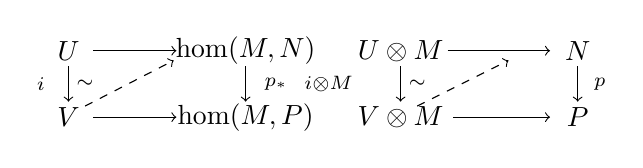
\begin{tikzpicture}[x=2.0em,y=1.6em]
  \node (U1) at (0,1.5) {$U$};
  \node (hMN) at (3.2,1.5) {$\mathrm{hom}(M,N)$};
  \node (V1) at (0,0) {$V$};
  \node (hMP) at (3.2,0) {$\mathrm{hom}(M,P)$};
  \draw[->] (0.45,1.5) -- (1.95,1.5);
  \draw[->] (0.45,0) -- (1.95,0);
  \draw[->] (0,1.15) -- (0,0.35);
  \node at (-0.5,0.75) {$\scriptstyle i$};
  \node at (0.3,0.75) {$\scriptstyle\sim$};
  \draw[->] (3.2,1.15) -- (3.2,0.35);
  \node at (3.75,0.75) {$\scriptstyle p_{\ast}$};
  \draw[->,dashed] (0.3,0.25) -- (1.9,1.28);
  \begin{scope}[shift={(6.0,0)}]
    \node (U2) at (0,1.5) {$U\otimes M$};
    \node (N2) at (3.2,1.5) {$N$};
    \node (V2) at (0,0) {$V\otimes M$};
    \node (P2) at (3.2,0) {$P$};
    \draw[->] (0.85,1.5) -- (2.7,1.5);
    \draw[->] (0.95,0) -- (2.7,0);
    \draw[->] (0,1.15) -- (0,0.35);
    \node at (-1.3,0.75) {$\scriptstyle i\otimes M$};
    \node at (0.3,0.75) {$\scriptstyle\sim$};
    \draw[->] (3.2,1.15) -- (3.2,0.35);
    \node at (3.6,0.75) {$\scriptstyle p$};
    \draw[->,dashed] (0.3,0.25) -- (1.95,1.28);
  \end{scope}
\end{tikzpicture}
\end{center}
由\cref{ex:quillen-bifunctor-component}，既然 $M$ 是\trCofibrant{}的，
$-\otimes M\colon\mathcal{V}\to\mathcal{M}$ 是左 Quillen 的，于是 $i\otimes M$
是 $\mathcal{M}$ 中的一支平凡余纤维化；又因 $p\colon N\rvFarrow P$ 是一支%
\trFibration，该\trLifting{}问题有解。
\end{proof}

下一个结果由 Gambino \cite{bib45} 在一个富集于 Quillen 的单纯集笛卡尔封闭模型结
构之上的\trModelCategory{}的语境中表述，但其证明适用于更大的普遍性。

\begin{theorem}\label{thm:weighted-colimit-limit-quillen}
若 $\mathcal{M}$ 是一个 $\mathcal{V}$-模型范畴且 $\mathcal{J}$ 是一个小范畴，则
加权\trColimit{}\trFunctor
\[ \operatorname{colim}_{--}\colon
   \mathcal{V}^{\mathcal{J}}\times\mathcal{M}^{\mathcal{J}^{\mathrm{op}}}
   \to\mathcal{M} \]
在诸定义域范畴具有（内射，射影）或（射影，内射）模型结构时是左 Quillen 的。类似
地，加权\trLimit{}\trFunctor
\[ \operatorname{lim}_{--}\colon
   (\mathcal{V}^{\mathcal{J}})^{\mathrm{op}}\times\mathcal{M}^{\mathcal{J}}
   \to\mathcal{M} \]
在诸定义域范畴具有（射影，射影）或（内射，内射）模型结构时是右 Quillen 的。
\end{theorem}
\begin{proof}
由\cref{def:quillen-two-variable-adjunction}，我们可以以\trAdjunction{}形式证明
这两个陈述。附录 A 中的\cref{def:weighted-limit-colimit-universal-property}的加
权\trColimit{}\trBifunctor{}容有一个\trRightAdjoint（它被用来表达加权%
\trColimit{}的定义性\trUniversalProperty）
\[ \mathrm{hom}\colon
   (\mathcal{M}^{\mathcal{J}^{\mathrm{op}}})^{\mathrm{op}}\times\mathcal{M}
   \to\mathcal{V}^{\mathcal{J}} \]
它把 $F\in\mathcal{M}^{\mathcal{J}^{\mathrm{op}}}$ 与 $m\in\mathcal{M}$ 送到
$\mathrm{hom}(F-,m)\in\mathcal{V}^{\mathcal{J}}$。

为证 $\mathcal{V}^{\mathcal{J}}$ 具有射影模型结构而
$\mathcal{M}^{\mathcal{J}^{\mathrm{op}}}$ 具有内射\trModelStructure{}时的那个陈述，我们必须
证明：这是一个相对于 $\mathcal{M}^{\mathcal{J}^{\mathrm{op}}}$ 中的逐点（平凡）余
纤维化、$\mathcal{M}$ 中的（平凡）\trFibration{}以及 $\mathcal{V}^{\mathcal{J}}$
中的逐点（平凡）\trFibration{}而言的右 Quillen \trBifunctor。由于右 Quillen %
\trBifunctor{}定义中所涉及的诸\trLimit{}也是逐点构成的，这立即由富集 hom %
\trBifunctor{}的相应性质得出——后者是富集模型范畴定义的一部分。其余诸情形类似。
\end{proof}

\begin{digression}[\trHomotopyColimit{}的构造]\label{dig:homotopy-colimit-construction}
在一个\trModelCategory{}中，术语\emph{\trHomotopyColimit}与\emph{\trHomotopyLimit}
指称\trColimit{}\trFunctor{}与\trLimit{}\trFunctor{}的导出函子。%
\cref{thm:weighted-colimit-limit-quillen}的要旨在于：构造一个%
\trHomotopyColimit{}有两条进路——「增肥\trDiagram」，例如要求其诸对象是%
\trCofibrant{}的且其诸态射是余纤维化——或者「增肥权」，典型做法是取终权的一个余
纤维性替换 \cite[§11.5]{bib103}。第 6 章中的\cref{lem:iso-commas-pullbacks}与%
\cref{lem:iso-towers-flexible}可以被理解为这两种进路之间的一般等价的实例。
\end{digression}

我们从\cref{thm:weighted-colimit-limit-quillen}的众多推论中单独挑出如下一条，其
令人感兴趣之处在于：第 6 章中的\cref{def:flexible-weights}的诸柔性权，恰好就是权
的范畴上相对于单纯集的 Joyal \trModelStructure{}而定义的射影模型结构中的诸%
\trCofibrant{}对象。

\begin{corollary}\label{cor:flexible-weight-fibrant-limit}
若 $\mathcal{M}$ 是一个 $\mathcal{V}$-模型范畴，则对任何对象皆为\trFibrant{}的%
\trDiagram{} $F\in\mathcal{M}^{\mathcal{J}}$ 与任何射影\trCofibrant{}的权
$W\in\mathcal{V}^{\mathcal{J}}$，加权\trLimit{}是一个\trFibrant{}对象。
\end{corollary}
\begin{proof}
由\cref{thm:weighted-colimit-limit-quillen}，加权\trLimit{}\trBifunctor%
$\operatorname{lim}_{--}\colon(\mathcal{V}^{\mathcal{J}})^{\mathrm{op}}\times\mathcal{M}^{\mathcal{J}}\to\mathcal{M}$ 相对于权的范畴上的射影模型结构与%
\trDiagram{}\trCategory{}上的射影模型结构是右 Quillen 的。既然右 Quillen %
\trBifunctor{}保持\trFibrant{}对象，由此得出：由一个射影\trCofibrant{}的权加权的%
\trPointwise{}纤维性图表之\trLimit{}是\trFibrant{}的。
\end{proof}

最后，我们将利用下述定理，它使\trModelCategory{}的富集\trChangeOfBase{}成为可能，
推广了 A.7 节的结果。\cref{thm:change-of-base-quillen-model}的前提是附录 A 中的%
\cref{prop:change-of-base-2-adjunction}的前提到富集模型范畴语境中的显然推广，但其
结论只容许我们沿\trRightAdjoint{}的方向转移富集，因为一个富集模型范畴还必须是张
量化且余张量化的，而这些性质只沿那个方向转移。

下面的结果是把 \cite[3.8]{bib50} 中所证明的一个更一般的定理特化到富集之笛卡尔封闭
基的情形。

\begin{theorem}\label{thm:change-of-base-quillen-model}
试考虑介于诸笛卡尔封闭的模型范畴之间的一个 Quillen \trAdjunction，其中%
\trLeftAdjoint{}保持有限积：
\begin{center}
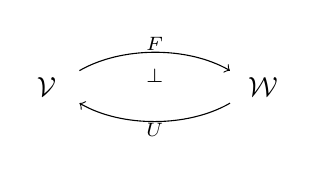
\begin{tikzpicture}[x=1.7em,y=1.4em]
  \node (V) at (0,0) {$\mathcal{V}$};
  \node (W) at (4.6,0) {$\mathcal{W}$};
  \draw[->] (0.7,0.42) .. controls (1.6,1.05) and (3.0,1.05) .. (3.9,0.42);
  \node at (2.3,1.12) {$\scriptstyle F$};
  \node at (2.3,0.28) {$\scriptstyle\bot$};
  \draw[->] (3.9,-0.42) .. controls (3.0,-1.05) and (1.6,-1.05) .. (0.7,-0.42);
  \node at (2.3,-1.12) {$\scriptstyle U$};
\end{tikzpicture}
\end{center}
那么，任何 $\mathcal{W}$-模型范畴都容有成为一个 $\mathcal{V}$-模型范畴的结构，
后者具有同一个底非富集模型范畴，其富集 hom、\trCotensor{}与\trTensor{}由下式
定义：
\[ \mathrm{hom}_{\mathcal{V}}(M,N)\coloneqq U\,\mathrm{hom}_{\mathcal{W}}(M,N),
   \qquad
   V\otimes M\coloneqq FV\otimes M,\qquad\text{以及}\qquad
   M^{V}\coloneqq M^{FV}. \]
\end{theorem}
\begin{proof}
由附录 A 中的\cref{prop:change-of-base-tensored-cotensored}，这些定义使
$\mathcal{M}$\footnote{原书印作「$\mathcal{W}$」，疑为「$\mathcal{M}$」之误——受换基富集者应为该 $\mathcal{W}$-模型范畴本身，此处径改。——译者注}成为一个张量化且余张量化的 $\mathcal{V}$-富集范畴。附录 A 中的%
\cref{lem:change-of-base-underlying-categories}观察到：沿保持有限积的%
\trAdjunction{}之\trRightAdjoint{}所作的换基保持诸底 1-\trCategory。尚须验证的
只是：$\mathcal{V}$-富集 hom、\trTensor{}与\trCotensor{}底下的诸\trFunctor{}定义
一个 Quillen
双变量\trAdjunction，而这容易由\trModelCategory{} $\mathcal{V}$ 与 $\mathcal{W}$ 的笛卡尔
封闭性以及 $F\dashv U$ 是 Quillen 的这一事实得出。
\end{proof}

\subsection*{练习}

\begin{exercise}\label{ex:fibrant-objects-from-model}
验证：一个\trModelCategory{}中\trFibrant{}对象的全子范畴定义一个\trCategoryOfFibrantObjects，
其中取 $\rvW$ 为\trWeakEquivalence{}类、取 $\rvF$ 为\trFibrant{}对象之间的诸%
\trFibration{}的类。
\end{exercise}

\begin{exercise}\label{ex:model-structure-determined}
验证：$\mathcal{M}$ 上的一个\trModelStructure（若它存在的话）由下列诸数据中的任
何一个唯一确定：
\begin{enumerate}[label=(\roman*)]
\item 余纤维化与\trWeakEquivalence；
\item \trFibration{}与\trWeakEquivalence；
\item 余纤维化与\trFibration；或者
\item 平凡余纤维化与\trTrivialFibration。%
  \footnote{据 Joyal 的一个更为精致的观察 \cite[E.1.10]{bib63}，模型结构还由如下
  数据唯一确定：(v) 余纤维化与纤维性对象，或 (vi) 纤维化与余纤维性对象。}
\end{enumerate}
\end{exercise}

\begin{exercise}\label{ex:quillen-bifunctor-component}
\begin{enumerate}[label=(\roman*)]
\item 证明：若 $\otimes\colon\mathcal{V}\times\mathcal{M}\to\mathcal{N}$ 是一个
  左 Quillen \trBifunctor{}且 $V\in\mathcal{V}$ 是\trCofibrant{}的，则
  $V\otimes-\colon\mathcal{M}\to\mathcal{N}$ 是一个左 Quillen \trFunctor。
\item 由此推论：若 $1\in\mathcal{V}$ 是\trCofibrant{}的，则%
  \cref{def:cartesian-closed-model-category}与\cref{def:v-model-category}的第二
  个条件是不必要的。
\end{enumerate}
\end{exercise}

\begin{exercise}\label{ex:set-model-category}
在一个带\trProduct{}与\trCoproduct{}的局部小范畴（locally small category）
$\mathcal{M}$ 中，hom \trBifunctor{}是某个双变量\trAdjunction{}的一部分：
\[ \ast\colon\mathcal{S}et\times\mathcal{M}\to\mathcal{M},\qquad
   \{,\}\colon\mathcal{S}et^{\mathrm{op}}\times\mathcal{M}\to\mathcal{M},\qquad
   \mathrm{hom}\colon\mathcal{M}^{\mathrm{op}}\times\mathcal{M}\to\mathcal{S}et. \]
为 $\mathcal{S}et$ 配备如下\trModelStructure——其\trWeakEquivalence{}是一切映
射、其余纤维化是诸\trMonomorphism、其\trFibration{}是诸\trEpimorphism——并证明：
\begin{enumerate}[label=(\roman*)]
\item $\mathcal{S}et$ 是一个笛卡尔封闭的模型范畴。
\item 任何\trModelCategory{} $\mathcal{M}$ 都是一个 $\mathcal{S}et$-模型范畴。
\end{enumerate}
\end{exercise}

